\documentclass[11pt]{article}
\usepackage{geometry}                % See geometry.pdf to learn the layout options. There are lots.
\geometry{letterpaper}                   % ... or a4paper or a5paper or ... 
%\geometry{landscape}                % Activate for for rotated page geometry
%\usepackage[parfill]{parskip}    % Activate to begin paragraphs with an empty line rather than an indent
\usepackage{graphicx}
\usepackage{amssymb,amsmath}
\usepackage{epstopdf}
\usepackage{pgf}
\usepackage{pgfpages}
\usepackage{tikz}
\usetikzlibrary{arrows,backgrounds}
\usepgflibrary{shapes}
\DeclareGraphicsRule{.tif}{png}{.png}{`convert #1 `dirname #1`/`basename #1 .tif`.png}
\pagestyle{empty}


\begin{document}

% Tetrahedron Node Numbering
  \begin{center}
    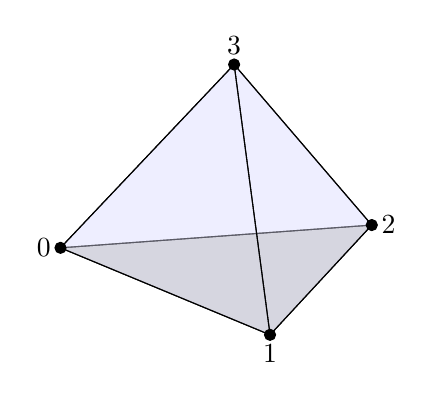
\begin{tikzpicture}[join=round] % tet with 4 nodes
        \filldraw[fill=black!20](1.748,.561)--(-2.205,.272)--(.456,-.833)--cycle;
        \filldraw[fill=blue!10,fill opacity=0.4](0,2.6)--(-2.205,.272)--(1.748,.561)--(0,2.6)--cycle;
        \filldraw[fill=blue!10,fill opacity=0.4](0,2.6)--(1.748,.561)--(.456,-.833)--(0,2.6)--cycle;
        \filldraw[fill=blue!10,fill opacity=0.4](0,2.6)--(.456,-.833)--(-2.205,.272)--(0,2.6)--cycle;
        \filldraw(1.748,.561) circle (2pt);
        \filldraw(-2.205,.272) circle (2pt);
        \filldraw(0,2.6) circle (2pt);
        \filldraw(.456,-.833) circle (2pt);
        \fill[black]
                (-2.205,.272) node [left] {0}
                (.456,-.833) node [below] {1}
                (1.748,.561) node [right] {2}
                (0,2.6) node [above] {3};
    \end{tikzpicture}
     \hspace{1cm}
    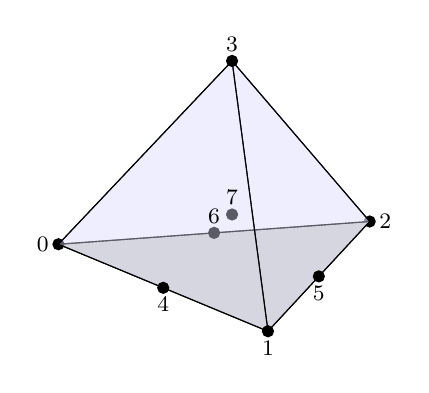
\begin{tikzpicture}[join=round] % tet with 8 nodes
        \filldraw(1.748,.561) circle (2pt);
        \filldraw[fill=black!20](1.748,.561)--(-2.205,.272)--(.456,-.833)--cycle;
        \filldraw[fill=blue!10,fill opacity=0.4](0,2.6)--(-2.205,.272)--(1.748,.561)--(0,2.6)--cycle;
        \filldraw[fill=blue!10,fill opacity=0.4](0,2.6)--(1.748,.561)--(.456,-.833)--(0,2.6)--cycle;
        \filldraw(-.228,.417) circle (2pt);
        \filldraw(-2.205,.272) circle (2pt);
        \filldraw(0,.65) circle (2pt);
        \filldraw[fill=blue!10,fill opacity=0.4](0,2.6)--(.456,-.833)--(-2.205,.272)--(0,2.6)--cycle;
        \filldraw(1.102,-.136) circle (2pt);
        \filldraw(-.874,-.281) circle (2pt);
        \filldraw(0,2.6) circle (2pt);
        \filldraw(.456,-.833) circle (2pt);
        \fill[black,font=\footnotesize]
                (-2.205,.272) node [left] {0}
                (.456,-.833) node [below] {1}
                (1.748,.561) node [right] {2}
                (0,2.6) node [above] {3}
                (-.874,-.281) node [below] {4}
                (1.102,-.136) node [below] {5}
                (-.228,.417) node [above] {6}
                (0,.65) node [above] {7};
     \end{tikzpicture}
   \end{center}
   \begin{center} {(a) \hspace{5cm} (b)}  \end{center}
   \begin{center}
    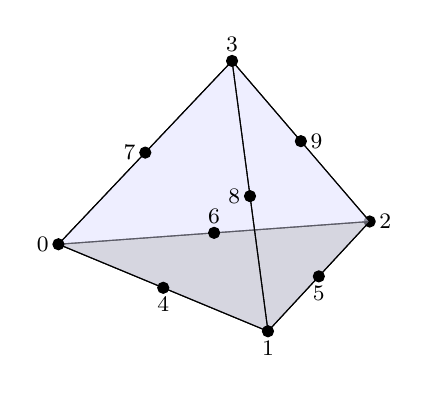
\begin{tikzpicture}[join=round]% tet with 10 nodes
        \filldraw[fill=black!20](1.748,.561)--(-2.205,.272)--(.456,-.833)--cycle;
        \filldraw(1.748,.561) circle (2pt);
        \filldraw[fill=blue!10,fill opacity=0.4](0,2.6)--(-2.205,.272)--(1.748,.561)--(0,2.6)--cycle;
        \filldraw[fill=blue!10,fill opacity=0.4](0,2.6)--(1.748,.561)--(.456,-.833)--(0,2.6)--cycle;
        \filldraw[fill=blue!10,fill opacity=0.4](0,2.6)--(.456,-.833)--(-2.205,.272)--(0,2.6)--cycle;
        \filldraw(-.228,.417) circle (2pt);
        \filldraw(-2.205,.272) circle (2pt);
        \filldraw(.874,1.581) circle (2pt);
        \filldraw(-1.102,1.436) circle (2pt);
        \filldraw(1.102,-.136) circle (2pt);
        \filldraw(-.874,-.281) circle (2pt);
        \filldraw(0,2.6) circle (2pt);
        \filldraw(.228,.883) circle (2pt);
        \filldraw(.456,-.833) circle (2pt);
        \fill[black,font=\footnotesize]
                (-2.205,.272) node [left] {0}
                (.456,-.833) node [below] {1}
                (1.748,.561) node [right] {2}
                (0,2.6) node [above] {3}
                (-.874,-.281) node [below] {4}
                (1.102,-.136) node [below] {5}
                (-.228,.417) node [above] {6}
                (-1.102,1.436) node [left] {7}
                (.228,.883) node [left] {8}
                (.874,1.581) node [right] {9};
     \end{tikzpicture}
    \end{center}
  \begin{center}
             (c) 
   \end{center}


\end{document}  
